\documentclass[10pt]{article} % For LaTeX2e
\usepackage{tmlr}
% If accepted, instead use the following line for the camera-ready submission:
%\usepackage[accepted]{tmlr}
% To de-anonymize and remove mentions to TMLR (for example for posting to preprint servers):
%\usepackage[preprint]{tmlr}

%%%%% NEW MATH DEFINITIONS %%%%%

\usepackage{amsmath,amsfonts,bm}

% Mark sections of captions for referring to divisions of figures
\newcommand{\figleft}{{\em (Left)}}
\newcommand{\figcenter}{{\em (Center)}}
\newcommand{\figright}{{\em (Right)}}
\newcommand{\figtop}{{\em (Top)}}
\newcommand{\figbottom}{{\em (Bottom)}}
\newcommand{\captiona}{{\em (a)}}
\newcommand{\captionb}{{\em (b)}}
\newcommand{\captionc}{{\em (c)}}
\newcommand{\captiond}{{\em (d)}}

% Highlight a newly defined term
\newcommand{\newterm}[1]{{\bf #1}}


% Figure reference, lower-case.
\def\figref#1{figure~\ref{#1}}
% Figure reference, capital. For start of sentence
\def\Figref#1{Figure~\ref{#1}}
\def\twofigref#1#2{figures \ref{#1} and \ref{#2}}
\def\quadfigref#1#2#3#4{figures \ref{#1}, \ref{#2}, \ref{#3} and \ref{#4}}
% Section reference, lower-case.
\def\secref#1{section~\ref{#1}}
% Section reference, capital.
\def\Secref#1{Section~\ref{#1}}
% Reference to two sections.
\def\twosecrefs#1#2{sections \ref{#1} and \ref{#2}}
% Reference to three sections.
\def\secrefs#1#2#3{sections \ref{#1}, \ref{#2} and \ref{#3}}
% Reference to an equation, lower-case.
\def\eqref#1{equation~\ref{#1}}
% Reference to an equation, upper case
\def\Eqref#1{Equation~\ref{#1}}
% A raw reference to an equation---avoid using if possible
\def\plaineqref#1{\ref{#1}}
% Reference to a chapter, lower-case.
\def\chapref#1{chapter~\ref{#1}}
% Reference to an equation, upper case.
\def\Chapref#1{Chapter~\ref{#1}}
% Reference to a range of chapters
\def\rangechapref#1#2{chapters\ref{#1}--\ref{#2}}
% Reference to an algorithm, lower-case.
\def\algref#1{algorithm~\ref{#1}}
% Reference to an algorithm, upper case.
\def\Algref#1{Algorithm~\ref{#1}}
\def\twoalgref#1#2{algorithms \ref{#1} and \ref{#2}}
\def\Twoalgref#1#2{Algorithms \ref{#1} and \ref{#2}}
% Reference to a part, lower case
\def\partref#1{part~\ref{#1}}
% Reference to a part, upper case
\def\Partref#1{Part~\ref{#1}}
\def\twopartref#1#2{parts \ref{#1} and \ref{#2}}

\def\ceil#1{\lceil #1 \rceil}
\def\floor#1{\lfloor #1 \rfloor}
\def\1{\bm{1}}
\newcommand{\train}{\mathcal{D}}
\newcommand{\valid}{\mathcal{D_{\mathrm{valid}}}}
\newcommand{\test}{\mathcal{D_{\mathrm{test}}}}

\def\eps{{\epsilon}}


% Random variables
\def\reta{{\textnormal{$\eta$}}}
\def\ra{{\textnormal{a}}}
\def\rb{{\textnormal{b}}}
\def\rc{{\textnormal{c}}}
\def\rd{{\textnormal{d}}}
\def\re{{\textnormal{e}}}
\def\rf{{\textnormal{f}}}
\def\rg{{\textnormal{g}}}
\def\rh{{\textnormal{h}}}
\def\ri{{\textnormal{i}}}
\def\rj{{\textnormal{j}}}
\def\rk{{\textnormal{k}}}
\def\rl{{\textnormal{l}}}
% rm is already a command, just don't name any random variables m
\def\rn{{\textnormal{n}}}
\def\ro{{\textnormal{o}}}
\def\rp{{\textnormal{p}}}
\def\rq{{\textnormal{q}}}
\def\rr{{\textnormal{r}}}
\def\rs{{\textnormal{s}}}
\def\rt{{\textnormal{t}}}
\def\ru{{\textnormal{u}}}
\def\rv{{\textnormal{v}}}
\def\rw{{\textnormal{w}}}
\def\rx{{\textnormal{x}}}
\def\ry{{\textnormal{y}}}
\def\rz{{\textnormal{z}}}

% Random vectors
\def\rvepsilon{{\mathbf{\epsilon}}}
\def\rvtheta{{\mathbf{\theta}}}
\def\rva{{\mathbf{a}}}
\def\rvb{{\mathbf{b}}}
\def\rvc{{\mathbf{c}}}
\def\rvd{{\mathbf{d}}}
\def\rve{{\mathbf{e}}}
\def\rvf{{\mathbf{f}}}
\def\rvg{{\mathbf{g}}}
\def\rvh{{\mathbf{h}}}
\def\rvu{{\mathbf{i}}}
\def\rvj{{\mathbf{j}}}
\def\rvk{{\mathbf{k}}}
\def\rvl{{\mathbf{l}}}
\def\rvm{{\mathbf{m}}}
\def\rvn{{\mathbf{n}}}
\def\rvo{{\mathbf{o}}}
\def\rvp{{\mathbf{p}}}
\def\rvq{{\mathbf{q}}}
\def\rvr{{\mathbf{r}}}
\def\rvs{{\mathbf{s}}}
\def\rvt{{\mathbf{t}}}
\def\rvu{{\mathbf{u}}}
\def\rvv{{\mathbf{v}}}
\def\rvw{{\mathbf{w}}}
\def\rvx{{\mathbf{x}}}
\def\rvy{{\mathbf{y}}}
\def\rvz{{\mathbf{z}}}

% Elements of random vectors
\def\erva{{\textnormal{a}}}
\def\ervb{{\textnormal{b}}}
\def\ervc{{\textnormal{c}}}
\def\ervd{{\textnormal{d}}}
\def\erve{{\textnormal{e}}}
\def\ervf{{\textnormal{f}}}
\def\ervg{{\textnormal{g}}}
\def\ervh{{\textnormal{h}}}
\def\ervi{{\textnormal{i}}}
\def\ervj{{\textnormal{j}}}
\def\ervk{{\textnormal{k}}}
\def\ervl{{\textnormal{l}}}
\def\ervm{{\textnormal{m}}}
\def\ervn{{\textnormal{n}}}
\def\ervo{{\textnormal{o}}}
\def\ervp{{\textnormal{p}}}
\def\ervq{{\textnormal{q}}}
\def\ervr{{\textnormal{r}}}
\def\ervs{{\textnormal{s}}}
\def\ervt{{\textnormal{t}}}
\def\ervu{{\textnormal{u}}}
\def\ervv{{\textnormal{v}}}
\def\ervw{{\textnormal{w}}}
\def\ervx{{\textnormal{x}}}
\def\ervy{{\textnormal{y}}}
\def\ervz{{\textnormal{z}}}

% Random matrices
\def\rmA{{\mathbf{A}}}
\def\rmB{{\mathbf{B}}}
\def\rmC{{\mathbf{C}}}
\def\rmD{{\mathbf{D}}}
\def\rmE{{\mathbf{E}}}
\def\rmF{{\mathbf{F}}}
\def\rmG{{\mathbf{G}}}
\def\rmH{{\mathbf{H}}}
\def\rmI{{\mathbf{I}}}
\def\rmJ{{\mathbf{J}}}
\def\rmK{{\mathbf{K}}}
\def\rmL{{\mathbf{L}}}
\def\rmM{{\mathbf{M}}}
\def\rmN{{\mathbf{N}}}
\def\rmO{{\mathbf{O}}}
\def\rmP{{\mathbf{P}}}
\def\rmQ{{\mathbf{Q}}}
\def\rmR{{\mathbf{R}}}
\def\rmS{{\mathbf{S}}}
\def\rmT{{\mathbf{T}}}
\def\rmU{{\mathbf{U}}}
\def\rmV{{\mathbf{V}}}
\def\rmW{{\mathbf{W}}}
\def\rmX{{\mathbf{X}}}
\def\rmY{{\mathbf{Y}}}
\def\rmZ{{\mathbf{Z}}}

% Elements of random matrices
\def\ermA{{\textnormal{A}}}
\def\ermB{{\textnormal{B}}}
\def\ermC{{\textnormal{C}}}
\def\ermD{{\textnormal{D}}}
\def\ermE{{\textnormal{E}}}
\def\ermF{{\textnormal{F}}}
\def\ermG{{\textnormal{G}}}
\def\ermH{{\textnormal{H}}}
\def\ermI{{\textnormal{I}}}
\def\ermJ{{\textnormal{J}}}
\def\ermK{{\textnormal{K}}}
\def\ermL{{\textnormal{L}}}
\def\ermM{{\textnormal{M}}}
\def\ermN{{\textnormal{N}}}
\def\ermO{{\textnormal{O}}}
\def\ermP{{\textnormal{P}}}
\def\ermQ{{\textnormal{Q}}}
\def\ermR{{\textnormal{R}}}
\def\ermS{{\textnormal{S}}}
\def\ermT{{\textnormal{T}}}
\def\ermU{{\textnormal{U}}}
\def\ermV{{\textnormal{V}}}
\def\ermW{{\textnormal{W}}}
\def\ermX{{\textnormal{X}}}
\def\ermY{{\textnormal{Y}}}
\def\ermZ{{\textnormal{Z}}}

% Vectors
\def\vzero{{\bm{0}}}
\def\vone{{\bm{1}}}
\def\vmu{{\bm{\mu}}}
\def\vtheta{{\bm{\theta}}}
\def\va{{\bm{a}}}
\def\vb{{\bm{b}}}
\def\vc{{\bm{c}}}
\def\vd{{\bm{d}}}
\def\ve{{\bm{e}}}
\def\vf{{\bm{f}}}
\def\vg{{\bm{g}}}
\def\vh{{\bm{h}}}
\def\vi{{\bm{i}}}
\def\vj{{\bm{j}}}
\def\vk{{\bm{k}}}
\def\vl{{\bm{l}}}
\def\vm{{\bm{m}}}
\def\vn{{\bm{n}}}
\def\vo{{\bm{o}}}
\def\vp{{\bm{p}}}
\def\vq{{\bm{q}}}
\def\vr{{\bm{r}}}
\def\vs{{\bm{s}}}
\def\vt{{\bm{t}}}
\def\vu{{\bm{u}}}
\def\vv{{\bm{v}}}
\def\vw{{\bm{w}}}
\def\vx{{\bm{x}}}
\def\vy{{\bm{y}}}
\def\vz{{\bm{z}}}

% Elements of vectors
\def\evalpha{{\alpha}}
\def\evbeta{{\beta}}
\def\evepsilon{{\epsilon}}
\def\evlambda{{\lambda}}
\def\evomega{{\omega}}
\def\evmu{{\mu}}
\def\evpsi{{\psi}}
\def\evsigma{{\sigma}}
\def\evtheta{{\theta}}
\def\eva{{a}}
\def\evb{{b}}
\def\evc{{c}}
\def\evd{{d}}
\def\eve{{e}}
\def\evf{{f}}
\def\evg{{g}}
\def\evh{{h}}
\def\evi{{i}}
\def\evj{{j}}
\def\evk{{k}}
\def\evl{{l}}
\def\evm{{m}}
\def\evn{{n}}
\def\evo{{o}}
\def\evp{{p}}
\def\evq{{q}}
\def\evr{{r}}
\def\evs{{s}}
\def\evt{{t}}
\def\evu{{u}}
\def\evv{{v}}
\def\evw{{w}}
\def\evx{{x}}
\def\evy{{y}}
\def\evz{{z}}

% Matrix
\def\mA{{\bm{A}}}
\def\mB{{\bm{B}}}
\def\mC{{\bm{C}}}
\def\mD{{\bm{D}}}
\def\mE{{\bm{E}}}
\def\mF{{\bm{F}}}
\def\mG{{\bm{G}}}
\def\mH{{\bm{H}}}
\def\mI{{\bm{I}}}
\def\mJ{{\bm{J}}}
\def\mK{{\bm{K}}}
\def\mL{{\bm{L}}}
\def\mM{{\bm{M}}}
\def\mN{{\bm{N}}}
\def\mO{{\bm{O}}}
\def\mP{{\bm{P}}}
\def\mQ{{\bm{Q}}}
\def\mR{{\bm{R}}}
\def\mS{{\bm{S}}}
\def\mT{{\bm{T}}}
\def\mU{{\bm{U}}}
\def\mV{{\bm{V}}}
\def\mW{{\bm{W}}}
\def\mX{{\bm{X}}}
\def\mY{{\bm{Y}}}
\def\mZ{{\bm{Z}}}
\def\mBeta{{\bm{\beta}}}
\def\mPhi{{\bm{\Phi}}}
\def\mLambda{{\bm{\Lambda}}}
\def\mSigma{{\bm{\Sigma}}}

% Tensor
\DeclareMathAlphabet{\mathsfit}{\encodingdefault}{\sfdefault}{m}{sl}
\SetMathAlphabet{\mathsfit}{bold}{\encodingdefault}{\sfdefault}{bx}{n}
\newcommand{\tens}[1]{\bm{\mathsfit{#1}}}
\def\tA{{\tens{A}}}
\def\tB{{\tens{B}}}
\def\tC{{\tens{C}}}
\def\tD{{\tens{D}}}
\def\tE{{\tens{E}}}
\def\tF{{\tens{F}}}
\def\tG{{\tens{G}}}
\def\tH{{\tens{H}}}
\def\tI{{\tens{I}}}
\def\tJ{{\tens{J}}}
\def\tK{{\tens{K}}}
\def\tL{{\tens{L}}}
\def\tM{{\tens{M}}}
\def\tN{{\tens{N}}}
\def\tO{{\tens{O}}}
\def\tP{{\tens{P}}}
\def\tQ{{\tens{Q}}}
\def\tR{{\tens{R}}}
\def\tS{{\tens{S}}}
\def\tT{{\tens{T}}}
\def\tU{{\tens{U}}}
\def\tV{{\tens{V}}}
\def\tW{{\tens{W}}}
\def\tX{{\tens{X}}}
\def\tY{{\tens{Y}}}
\def\tZ{{\tens{Z}}}


% Graph
\def\gA{{\mathcal{A}}}
\def\gB{{\mathcal{B}}}
\def\gC{{\mathcal{C}}}
\def\gD{{\mathcal{D}}}
\def\gE{{\mathcal{E}}}
\def\gF{{\mathcal{F}}}
\def\gG{{\mathcal{G}}}
\def\gH{{\mathcal{H}}}
\def\gI{{\mathcal{I}}}
\def\gJ{{\mathcal{J}}}
\def\gK{{\mathcal{K}}}
\def\gL{{\mathcal{L}}}
\def\gM{{\mathcal{M}}}
\def\gN{{\mathcal{N}}}
\def\gO{{\mathcal{O}}}
\def\gP{{\mathcal{P}}}
\def\gQ{{\mathcal{Q}}}
\def\gR{{\mathcal{R}}}
\def\gS{{\mathcal{S}}}
\def\gT{{\mathcal{T}}}
\def\gU{{\mathcal{U}}}
\def\gV{{\mathcal{V}}}
\def\gW{{\mathcal{W}}}
\def\gX{{\mathcal{X}}}
\def\gY{{\mathcal{Y}}}
\def\gZ{{\mathcal{Z}}}

% Sets
\def\sA{{\mathbb{A}}}
\def\sB{{\mathbb{B}}}
\def\sC{{\mathbb{C}}}
\def\sD{{\mathbb{D}}}
% Don't use a set called E, because this would be the same as our symbol
% for expectation.
\def\sF{{\mathbb{F}}}
\def\sG{{\mathbb{G}}}
\def\sH{{\mathbb{H}}}
\def\sI{{\mathbb{I}}}
\def\sJ{{\mathbb{J}}}
\def\sK{{\mathbb{K}}}
\def\sL{{\mathbb{L}}}
\def\sM{{\mathbb{M}}}
\def\sN{{\mathbb{N}}}
\def\sO{{\mathbb{O}}}
\def\sP{{\mathbb{P}}}
\def\sQ{{\mathbb{Q}}}
\def\sR{{\mathbb{R}}}
\def\sS{{\mathbb{S}}}
\def\sT{{\mathbb{T}}}
\def\sU{{\mathbb{U}}}
\def\sV{{\mathbb{V}}}
\def\sW{{\mathbb{W}}}
\def\sX{{\mathbb{X}}}
\def\sY{{\mathbb{Y}}}
\def\sZ{{\mathbb{Z}}}

% Entries of a matrix
\def\emLambda{{\Lambda}}
\def\emA{{A}}
\def\emB{{B}}
\def\emC{{C}}
\def\emD{{D}}
\def\emE{{E}}
\def\emF{{F}}
\def\emG{{G}}
\def\emH{{H}}
\def\emI{{I}}
\def\emJ{{J}}
\def\emK{{K}}
\def\emL{{L}}
\def\emM{{M}}
\def\emN{{N}}
\def\emO{{O}}
\def\emP{{P}}
\def\emQ{{Q}}
\def\emR{{R}}
\def\emS{{S}}
\def\emT{{T}}
\def\emU{{U}}
\def\emV{{V}}
\def\emW{{W}}
\def\emX{{X}}
\def\emY{{Y}}
\def\emZ{{Z}}
\def\emSigma{{\Sigma}}

% entries of a tensor
% Same font as tensor, without \bm wrapper
\newcommand{\etens}[1]{\mathsfit{#1}}
\def\etLambda{{\etens{\Lambda}}}
\def\etA{{\etens{A}}}
\def\etB{{\etens{B}}}
\def\etC{{\etens{C}}}
\def\etD{{\etens{D}}}
\def\etE{{\etens{E}}}
\def\etF{{\etens{F}}}
\def\etG{{\etens{G}}}
\def\etH{{\etens{H}}}
\def\etI{{\etens{I}}}
\def\etJ{{\etens{J}}}
\def\etK{{\etens{K}}}
\def\etL{{\etens{L}}}
\def\etM{{\etens{M}}}
\def\etN{{\etens{N}}}
\def\etO{{\etens{O}}}
\def\etP{{\etens{P}}}
\def\etQ{{\etens{Q}}}
\def\etR{{\etens{R}}}
\def\etS{{\etens{S}}}
\def\etT{{\etens{T}}}
\def\etU{{\etens{U}}}
\def\etV{{\etens{V}}}
\def\etW{{\etens{W}}}
\def\etX{{\etens{X}}}
\def\etY{{\etens{Y}}}
\def\etZ{{\etens{Z}}}

% The true underlying data generating distribution
\newcommand{\pdata}{p_{\rm{data}}}
% The empirical distribution defined by the training set
\newcommand{\ptrain}{\hat{p}_{\rm{data}}}
\newcommand{\Ptrain}{\hat{P}_{\rm{data}}}
% The model distribution
\newcommand{\pmodel}{p_{\rm{model}}}
\newcommand{\Pmodel}{P_{\rm{model}}}
\newcommand{\ptildemodel}{\tilde{p}_{\rm{model}}}
% Stochastic autoencoder distributions
\newcommand{\pencode}{p_{\rm{encoder}}}
\newcommand{\pdecode}{p_{\rm{decoder}}}
\newcommand{\precons}{p_{\rm{reconstruct}}}

\newcommand{\laplace}{\mathrm{Laplace}} % Laplace distribution

\newcommand{\E}{\mathbb{E}}
\newcommand{\Ls}{\mathcal{L}}
\newcommand{\R}{\mathbb{R}}
\newcommand{\emp}{\tilde{p}}
\newcommand{\lr}{\alpha}
\newcommand{\reg}{\lambda}
\newcommand{\rect}{\mathrm{rectifier}}
\newcommand{\softmax}{\mathrm{softmax}}
\newcommand{\sigmoid}{\sigma}
\newcommand{\softplus}{\zeta}
\newcommand{\KL}{D_{\mathrm{KL}}}
\newcommand{\Var}{\mathrm{Var}}
\newcommand{\standarderror}{\mathrm{SE}}
\newcommand{\Cov}{\mathrm{Cov}}
% Wolfram Mathworld says $L^2$ is for function spaces and $\ell^2$ is for vectors
% But then they seem to use $L^2$ for vectors throughout the site, and so does
% wikipedia.
\newcommand{\normlzero}{L^0}
\newcommand{\normlone}{L^1}
\newcommand{\normltwo}{L^2}
\newcommand{\normlp}{L^p}
\newcommand{\normmax}{L^\infty}

\newcommand{\parents}{Pa} % See usage in notation.tex. Chosen to match Daphne's book.

\DeclareMathOperator*{\argmax}{arg\,max}
\DeclareMathOperator*{\argmin}{arg\,min}

\DeclareMathOperator{\sign}{sign}
\DeclareMathOperator{\Tr}{Tr}
\let\ab\allowbreak


\usepackage{hyperref}
\usepackage{url}
\usepackage{booktabs}
\usepackage{graphicx}
\usepackage{amsmath}
\usepackage{multirow}

\title{Domain-Complete Evaluation of Distribution Shift\\in Histopathology}

\author{\name Ayan Chatterjee$^{\dagger}$ \email ayanchatterjee@iitbbs.ac.in \\
      \addr School of Basic Sciences \\
      Indian Institute of Technology Bhubaneswar, India \\
      {\normalfont\footnotesize $^{\dagger}$Corresponding author}
      \AND
      \name Amitava Mukherjee \email amitava@dubai.bits-pilani.ac.in \\
      \addr Department of Mathematics \\
      Birla Institute of Technology \& Science, Pilani -- Dubai Campus, UAE}

\def\month{MM}
\def\year{YYYY}
\def\openreview{\url{https://openreview.net/forum?id=XXXX}}

\begin{document}

\maketitle

\begin{abstract}
When a pathology AI model trained at one hospital is deployed at another, it
often fails---not because it lacks capacity, but because each hospital's
scanner, staining protocol and patient population leave visual fingerprints
that the model confuses with disease. We investigate what actually governs
cross-domain generalization by testing eleven robustness methods across three
cohorts that isolate different sources of shift: Camelyon17-WILDS (five
hospitals, where scanner, stain and patients all change), MIDOG 2021 (three
scanners in one laboratory, where only the device changes), and a multi-scanner
canine cohort (five scanners, same slides). The central finding is that the
\emph{type} of domain shift---not just its presence---determines which method
works. Under full hospital shift, self-supervised pre-training on unlabelled
tissue lifts the worst hospital's AUROC by $0.175$ and compresses the
across-hospital spread threefold; under scanner-only shift, stain normalization
dominates instead and pre-training adds nothing. Most domain-generalization
objectives (GroupDRO, IRM, DeepCORAL) fail the worst domain on every cohort. A
frozen ImageNet linear probe outperforms all trained-from-scratch arms under
hospital shift, indicating that representation quality is a stronger lever than
any robustness objective at this model scale.

To make these comparisons rigorous, we propose using the intraclass correlation
coefficient ($\mathrm{ICC}_{\mathrm{site}}$) from a variance decomposition of
off-site performance as a quantitative measure of how much of a model's
variability is truly site-driven versus noise from random initialization. On
the baseline, hospital identity accounts for $55\%$ of variance; on the best
arm it accounts for $84\%$---meaning the intervention removed the noise floor
and left only systematic site structure. We derive the resulting power formula
and show that detecting a $0.10$ AUROC improvement requires at least eight
hospitals at three seeds, far more than current benchmarks provide.

For teams developing pathology AI for clinical deployment, the practical
implication is that robustness evaluation must be \emph{domain-complete} (test
at every available site), \emph{shift-aware} (know whether you face a scanner
change, a protocol change, or a full institutional change), and
\emph{seed-replicated} (run multiple seeds to separate real effects from
noise). We release the full protocol, all 388 experimental records, and the
code to reproduce every result.
\end{abstract}

\section{Introduction}

A model trained on slides from one set of hospitals tends to fail at a hospital
it has not seen. Each hospital's scanner, staining chemistry and patient mix
leave fingerprints on the tissue image, and a classifier is free to learn those
fingerprints whenever they happen to correlate with the diagnosis
\citep{zech2018variable,geirhos2020shortcut}. In histopathology the hospital
signal is so strong that hospital identity alone is predictable from slide
appearance with near-perfect accuracy \citep{howard2021site}, and the practical
consequence is well documented: most models that undergo external validation
lose accuracy \citep{yu2022external}.

Many methods have been proposed to fix this---from domain-invariant training
objectives to stain normalization to self-supervised pre-training---but the way
they are evaluated has not kept up. A typical paper tests its fix at one
held-out hospital, because that is what the standard benchmark provides: the
official Camelyon17-WILDS split \citep{koh2021wilds} designates a single
centre as the out-of-distribution test set, and the leaderboard ranks methods
by their accuracy there. If your model happens to do well at that particular
hospital, the method looks good. If the hospital is an easy one, every method
looks good.

This paper asks a simple question: \emph{what happens when you test at every
hospital instead of just one?} We hold out each of the five Camelyon17 centres
in turn, run eleven robustness interventions through one shared training
pipeline with three random seeds per core arm, and then repeat the whole
experiment on two additional cohorts where only the scanner changes. The
backbone is deliberately small ($0.58$\,M parameters at $64\times64$
resolution) so that the complete grid---180 GPU jobs---finishes in 32 minutes
on one GPU. Any laboratory that can afford a single ablation study can afford
this one.

\paragraph{Contributions.}

\begin{enumerate}
\item \textbf{Shift-type-dependent method selection}
(\S\ref{sec:eleven}, \S\ref{sec:cohorts}). We show that the dominant source
of domain shift---scanner hardware, staining protocol, or full institutional
change---determines which robustness method works. Under hospital shift
(scanner + stain + patients), self-supervised pre-training lifts the worst
hospital's AUROC by $0.175$ and compresses cross-hospital spread $3.2\times$;
under scanner-only shift, stain normalization dominates instead, and
pre-training adds nothing. Most domain-generalization objectives (GroupDRO,
IRM, DeepCORAL) hurt the worst domain on every cohort. A frozen ImageNet probe
outperforms all trained-from-scratch arms under hospital shift, establishing
representation quality as the primary lever at this model scale
(\S\ref{sec:ssl}, \S\ref{sec:pcam}).

\item \textbf{A variance-decomposition framework for evaluating robustness
claims} (\S\ref{sec:variance}). We propose using the intraclass correlation
coefficient $\mathrm{ICC}_{\mathrm{site}}$, estimated from a two-way
random-effects model, to quantify how much of a model's performance variability
is genuinely site-driven versus initialization noise. We derive a closed-form
power formula showing that detecting a $0.10$ AUROC mean effect requires at
least eight hospitals at three seeds---far beyond what standard single-site
evaluations provide. This gives the field a principled tool for deciding when a
robustness claim is statistically supported.

\item \textbf{A domain-complete evaluation protocol for clinical AI
deployment} (\S\ref{sec:protocol}). We operationalize these findings into a
concrete protocol: evaluate at every available domain, report worst-domain
performance and across-domain spread, replicate seeds, and use the ICC
decomposition to verify that the evaluation grid has sufficient power before
publishing a robustness claim. At compact-model scale the complete protocol
costs under one hour of GPU time.
\end{enumerate}

All 388 experimental records and the code to regenerate every table and figure
are publicly released.

\section{Related work}

\paragraph{Site effects in medical imaging.} That acquisition site drives model
behaviour is established across modalities
\citep{zech2018variable,yu2022external}. \citet{howard2021site} showed for
histopathology specifically that site signatures are recoverable from slide
appearance and that they bias downstream predictions. Our contribution is not
the existence of the effect but its magnitude relative to method effects when
both are measured under one protocol.

\paragraph{Domain generalization and the WILDS benchmark.}
Camelyon17-WILDS \citep{koh2021wilds,bandi2019camelyon17} is the standard
testbed for cross-hospital shift. Methods evaluated on it include group
distributionally robust optimization \citep{sagawa2020groupdro}, invariant risk
minimization \citep{arjovsky2019irm}, deep feature-covariance alignment
\citep{sun2016coral}, style mixing \citep{zhou2021mixstyle}, gradient matching
\citep{shi2022fish} and selective augmentation \citep{yao2022lisa}. Each is
reported at the benchmark's single out-of-distribution test centre. We
re-implement six of them inside our pipeline and run each at all five centres.

\paragraph{Self-supervision and augmentation in histopathology.} Contrastive
pre-training on unlabelled tissue is an established recipe in computational
pathology \citep{ciga2022ssl}, as is aggressive stain-space augmentation
\citep{tellez2019stain} and classical stain normalization
\citep{macenko2009}. We make no claim of methodological novelty for the SimCLR
arm \citep{chen2020simclr}; the claim is about what a site-complete evaluation
reveals about it relative to the alternatives. Pathology foundation models
\citep{chen2024uni} operate two or more orders of magnitude above our scale;
\S\ref{sec:discussion} discusses what that means for our conclusions.

\paragraph{Variance in benchmarks.} \citet{bouthillier2021variance} argued that
machine-learning benchmarks under-report sources of variance and that
conclusions often do not survive accounting for them. Our variance
decomposition is an instance of that programme for one concrete clinical
benchmark, with the twist that one of the variance sources, hospital identity,
is also the quantity of scientific interest.

\section{The site-complete evaluation}
\label{sec:protocol}

\paragraph{Protocol.} Camelyon17-WILDS supplies $96\times96$ lymph-node patches
from five hospitals, labelled for tumour in the central $32\times32$ region;
we centre-crop to $64\times64$. For each fold $t \in \{0,\dots,4\}$ we hold out
centre $t$ as the off-site test hospital, use centre $v=(t-1)\bmod 5$ as the
out-of-distribution validation hospital for epoch selection, and train on the
remaining three centres. Each fold draws $30{,}000$ class-stratified training
patches, up to $12{,}000$ in-distribution validation patches, $12{,}000$
out-of-distribution validation patches and $25{,}000$ off-site test patches,
matching the official WILDS budget; $40{,}000$ further patches from the
training centres are held out unlabelled for pre-training. Every fold is
verified patient-disjoint across all roles, and each fold's self-supervised
encoder sees only that fold's own unlabelled pool, so no model is ever
pre-trained on tissue from its own test hospital. Fold $t=4$ (train
$\{0,1,2\}$, validate on $3$, test on $4$) reproduces the official WILDS
Camelyon17 split exactly, which lets us locate the benchmark's canonical
configuration inside the grid.

\paragraph{What to report.} A $K$-hospital grid supports some summaries better
than others. We report three. The \emph{worst-site} value is the AUROC at the
hospital where the arm does worst; it is the statistic a deployment decision
actually consumes, and it is well defined for any $K$. The \emph{across-site
standard deviation} measures how much the choice of hospital still matters once
the intervention is applied. The \emph{mean across sites} is the conventional
summary, and we report it with a paired-across-hospitals confidence interval
together with the number of hospitals that interval would need to be
informative at a given effect size (\S\ref{sec:variance}).

\section{Experimental setup}
\label{sec:setup}

All non-probe arms share one backbone: four convolutional stages of width
$32/64/128/256$ with batch normalization, global average pooling and a linear
classifier, $583{,}394$ parameters in total. All share one fine-tuning
schedule: SGD with momentum $0.9$, cosine learning rate from $0.02$, weight
decay $10^{-4}$, batch size $128$, five epochs, with the epoch chosen by
out-of-distribution validation AUROC. No per-arm hyperparameter tuning was
performed; every method uses its authors' recommended defaults. The arms are:

\begin{itemize}
\item \textbf{ERM} --- the supervised baseline.
\item \textbf{SAM} --- sharpness-aware minimization \citep{foret2021sam} at
$\rho=0.05$, batch-norm statistics frozen on the ascent step.
\item \textbf{SSL} (ours) --- a SimCLR encoder \citep{chen2020simclr}
pre-trained on the fold's own unlabelled pool with NT-Xent loss at temperature
$0.5$, batch size $256$, six epochs, H\&E-style colour and stain jitter,
followed by the shared supervised fine-tune.
\item \textbf{SSL+SAM} (ours) --- the same encoder, fine-tuned with SAM.
\item Four domain-generalization objectives: \textbf{GroupDRO}
\citep{sagawa2020groupdro} at $\eta=0.01$, \textbf{DeepCORAL}
\citep{sun2016coral} at $\lambda=1$, \textbf{IRMv1} \citep{arjovsky2019irm} at
$\lambda=1$ annealed from epoch 2, and \textbf{MixStyle}
\citep{zhou2021mixstyle} at $p=0.5,\alpha=0.1$ after stage 2. Hospital identity
supplies the group/domain label.
\item \textbf{Macenko + ERM} --- stain normalization \citep{macenko2009} fitted
on a 64-tile reference sample from the training set and applied to every input.
\item Three methods from the WILDS leaderboard: \textbf{Fish}
\citep{shi2022fish} with meta-learning rate $0.1$ and hospital-grouped inner
steps, \textbf{LISA} \citep{yao2022lisa} with same-class inter-hospital
$\mathrm{Beta}(2,2)$ mix-up, and \textbf{ERM + H\&E jitter}, aggressive
colour/brightness/hue jitter in H\&E space at strength $0.4$, following the
augmentation-only robustness strategy of \citet{tellez2019stain} and in the
spirit of the strong-augmentation baselines of \citet{taori2020robustness}.
\item \textbf{Frozen probe} --- a linear head on the frozen $2048$-d
penultimate features of a torchvision ResNet50 \citep{he2016resnet} pre-trained
on ImageNet-1K \citep{deng2009imagenet}, inputs bilinearly upsampled to
$224\times224$, head trained 15 epochs under the same selection rule.
\item Two further arms, used on the scanner cohorts of \S\ref{sec:cohorts},
reproduce the published top performers on those data: \textbf{TIA-style}, the
stain normalization plus heavy colour and dihedral augmentation of the
classification stage of the MIDOG-winning pipeline
\citep{jahanifar2024mitosis}, and \textbf{RotInv}, the dihedral invariance and
hard-negative strategy of \citet{lafarge2021rotation}.
\end{itemize}

The four core arms (ERM, SAM, SSL, SSL+SAM) are run at three seeds per fold;
the remaining seven at one seed per fold. We report AUROC, average precision,
accuracy, F1 and expected calibration error over 15 equal-width bins
\citep{naeini2015ece,guo2017calibration}. The Camelyon17 grid comes to $15$
self-supervised pre-training jobs, $105$ supervised training runs and $60$
PatchCamelyon checkpoint evaluations: $180$ GPU jobs, $0.53$ H100-hours. With
the two scanner cohorts of \S\ref{sec:cohorts} the study totals $388$ GPU jobs
and $1.23$ H100-hours.

\section{Results}

The results tell a story in three parts. We first show the full picture of
which methods survive testing at all five hospitals and which do not
(\S\ref{sec:eleven}), then look closely at why self-supervised pre-training
works where others fail (\S\ref{sec:ssl}--\ref{sec:pcam}), and finally reveal
that the entire ranking flips when we change what kind of shift the model
faces (\S\ref{sec:cohorts}). We close with the practical design question of
how many hospitals and random seeds a reliable evaluation actually requires
(\S\ref{sec:variance}).

%% ----------------------------------------------------------------
%% 5.1  THE HEADLINE: most methods fail
%% ----------------------------------------------------------------
\subsection{Most interventions fail domain-complete evaluation}
\label{sec:eleven}

The first thing the domain-complete grid reveals is how much the test hospital
matters. The supervised baseline's off-site AUROC runs from $0.724$ at
centre~2 to $0.920$ at centre~0---a spread of $0.196$ produced by the choice
of test hospital alone (Figure~\ref{fig:grid}a). Every method contrast in the
study is smaller than that spread. A report at centre~0 would describe the
baseline as strong; a report at centre~2 would describe the same pipeline on
the same data as barely usable. The official WILDS split (fold~4) sits at
$0.784$, neither the best nor the worst draw.

Table~\ref{tab:eleven} places all thirteen arms on the same grid, ordered by
worst-site AUROC; Figure~\ref{fig:grid}b plots the two primary summaries
against each other. Three patterns emerge.

\begin{table}[t]
\centering
\caption{Thirteen arms under the site-complete evaluation, ordered by
worst-site AUROC. Seed SD is the mean over folds of the within-fold seed
standard deviation, available only for the multi-seed arms. $r$ is the
correlation between per-hospital gain over ERM and per-hospital ERM AUROC;
$r_0$ is its value under independence (Appendix~\ref{app:shape}); the
informative quantity is the excess $r-r_0$. ECE is averaged over hospitals.}
\label{tab:eleven}
\small
\setlength{\tabcolsep}{4pt}
\begin{tabular}{lcccccccc}
\toprule
Arm & Worst site & Across-site SD & Mean & Seed SD & ECE & $r$ & $r_0$ & $r - r_0$ \\
\midrule
Frozen probe (IN-1K)          & $\mathbf{0.929}$ & $\mathbf{0.019}$ & $\mathbf{0.949}$ & --- & $\mathbf{0.022}$ & $-0.98$ & $-0.98$ & $-0.00$ \\
SSL (ours)                    & $0.899$ & $0.026$ & $0.933$ & $0.021$ & $0.073$ & $-0.95$ & $-0.96$ & $+0.00$ \\
SSL+SAM (ours)                & $0.894$ & $0.028$ & $0.941$ & $\mathbf{0.009}$ & $0.045$ & $-0.96$ & $-0.95$ & $-0.01$ \\
ERM + H\&E jitter             & $0.871$ & $0.042$ & $0.944$ & --- & $0.041$ & $-0.89$ & $-0.89$ & $+0.00$ \\
\midrule
MixStyle                      & $0.772$ & $0.070$ & $0.872$ & --- & $0.202$ & $-0.56$ & $-0.77$ & $+0.21$ \\
SAM                           & $0.726$ & $0.074$ & $0.828$ & $0.084$ & $0.185$ & $-0.69$ & $-0.75$ & $+0.06$ \\
ERM baseline                  & $0.724$ & $0.083$ & $0.838$ & $0.054$ & $0.187$ & --- & --- & --- \\
GroupDRO                      & $0.690$ & $0.095$ & $0.813$ & --- & $0.188$ & $+0.71$ & $-0.66$ & $+1.37$ \\
DeepCORAL                     & $0.683$ & $0.101$ & $0.814$ & --- & $0.179$ & $-0.12$ & $-0.64$ & $+0.51$ \\
IRMv1                         & $0.673$ & $0.103$ & $0.772$ & --- & $0.229$ & $-0.28$ & $-0.63$ & $+0.35$ \\
Macenko + ERM                 & $0.660$ & $0.107$ & $0.825$ & --- & $0.195$ & $-0.15$ & $-0.62$ & $+0.46$ \\
Fish                          & $0.533$ & $0.205$ & $0.689$ & --- & $0.273$ & $+0.60$ & $-0.38$ & $+0.97$ \\
LISA                          & $0.505$ & $0.162$ & $0.761$ & --- & $0.281$ & $-0.54$ & $-0.46$ & $-0.09$ \\
\bottomrule
\end{tabular}
\end{table}

\begin{figure}[t]
\centering
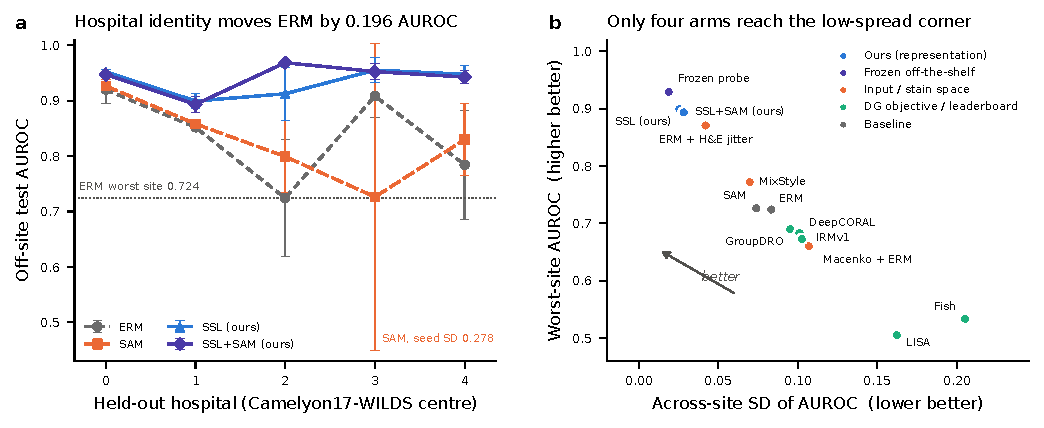
\includegraphics[width=\linewidth]{figs/fig1_site_complete}
\caption{\textbf{(a)} Off-site AUROC at each held-out hospital, mean over three
seeds, error bars one seed standard deviation. The supervised baseline swings
$0.196$ AUROC across hospitals; the pre-trained arms are nearly flat. SAM's
error bar at centre 3 spans $0.278$ AUROC, so seed noise alone, at one
hospital, exceeds the entire site range of the baseline. \textbf{(b)} All
thirteen arms in the worst-site / across-site-spread plane. Only the frozen
probe, the two pre-trained arms and H\&E jitter reach the low-spread corner.}
\label{fig:grid}
\end{figure}

First, only four of the ten alternatives improve the worst hospital at all: the
frozen probe ($0.929$), H\&E-space input jitter ($0.871$), MixStyle ($0.772$),
and SAM by $0.002$ AUROC, which is noise. The other six leave the worst
hospital \emph{below} the supervised baseline, among them three of the four
domain-generalization objectives, classical stain normalization, and both
leaderboard methods other than H\&E jitter. Under this protocol the two
families that work are representation-space pre-training and input-space
augmentation, and they work to comparable degrees. ERM with H\&E jitter reaches
worst-site $0.871$ and mean $0.944$, close to SSL+SAM, with no pre-training
stage at all. That favours the simpler method, and we report it as such.

Second, the spread the single-centre convention hides can be very large. Fish
ranges from $0.533$ to $0.919$ AUROC across the five hospitals of one cohort,
and LISA from $0.505$ to $0.906$. A number reported at one centre for either
method describes that centre. It is worth being careful about what this does
and does not show. Our re-implementations run inside a $0.58$\,M-parameter,
five-epoch pipeline rather than the authors' own, and Fish's
out-of-distribution validation curve selects epoch 1 in four of five folds
(Figure~\ref{fig:supp_epoch}), which is as much a model-selection pathology as
a method failure. What we are claiming is that these methods are highly
sensitive to which hospital is held out, not that these are the best numbers
they can reach.

Third, a linear probe on a frozen ImageNet-1K ResNet50 beats every
trained-from-scratch arm on every statistic in the table: worst-site $0.929$,
across-site SD $0.019$, mean $0.949$, ECE $0.022$. It does so after 22 seconds
of head-only training per fold, with no augmentation and no pathology-specific
supervision. This is not a pathology-foundation-model result and we do not
present it as one. It is a reference point: one step up in representation
quality leaves the hospital-to-hospital range nearly flat, which is what the
site-shortcut account predicts a sufficiently general representation should do,
and it sets a bar that none of the eleven trained-from-scratch interventions
clears.

The last three columns of Table~\ref{tab:eleven} address whether the arms that
do help target the hospitals that need it most. A large negative correlation
$r$ between a method's per-hospital gain and the baseline's per-hospital AUROC
looks like evidence of such targeting, but the statistic is mechanically
negative for any arm that is flatter than the baseline. For per-hospital
performance that is statistically independent of the baseline's,
\begin{equation}
r_0 = \frac{-\sigma_E}{\sqrt{\sigma_M^2 + \sigma_E^2}},
\label{eq:null}
\end{equation}
where $\sigma_E$ and $\sigma_M$ are the across-site standard deviations of the
baseline and method respectively; an arm that is simply uniform
($\sigma_M \to 0$) has $r_0 \to -1$ with no targeting. The excess $r - r_0$
removes this artifact. Our pre-trained arms sit at zero excess---they are
uniformly better, not selectively repairing the hard hospitals. GroupDRO
($+1.37$) and Fish ($+0.97$) show the opposite: they concentrate what gain
they have at the hospitals the baseline already handles. The full derivation
and per-arm response curves are in Appendix~\ref{app:shape}.

%% ----------------------------------------------------------------
%% 5.2  WHAT WORKS: SSL detail
%% ----------------------------------------------------------------
\subsection{Self-supervised pre-training compresses both nuisances}
\label{sec:ssl}

Table~\ref{tab:grid} breaks the four core arms out by hospital with three seeds
per cell. The pre-trained arms stand out from the grid above: they behave the
way a site-robustness intervention should. SSL raises the worst hospital from
$0.724$ to $0.899$ AUROC ($+0.175$) and compresses the across-site standard
deviation from $0.083$ to $0.026$, a $3.2\times$ reduction; the range across
hospitals falls from $0.196$ to $0.056$. The mean effect is $+0.096$ AUROC with
a paired-across-hospitals 95\% confidence interval of $[+0.004, +0.188]$
($t_4=2.89$, $p=0.045$). That is significant, but by a margin that
Table~\ref{tab:power} says we should not lean on at $K=5$, so we lean instead
on the worst-site and spread numbers, which are large and consistent.

\begin{table}[t]
\centering
\caption{The core grid: off-site test AUROC at each held-out hospital, mean
over three seeds $\pm$ the within-cell seed standard deviation. $\delta$
columns are differences from the ERM cell of the same hospital;
$I = \delta_{\mathrm{SSL+SAM}} - \delta_{\mathrm{SSL}} - \delta_{\mathrm{SAM}}$
is the interaction. Fold 4 is the official WILDS split.}
\label{tab:grid}
\small
\begin{tabular}{lccccccc}
\toprule
Held-out & ERM & SAM & SSL & SSL+SAM
& $\delta_{\mathrm{SSL}}$ & $\delta_{\mathrm{SAM}}$ & $I$ \\
\midrule
centre 0 & $0.920${\scriptsize$\pm.025$} & $0.927${\scriptsize$\pm.012$} & $0.952${\scriptsize$\pm.004$} & $0.947${\scriptsize$\pm.002$} & $+0.032$ & $+0.007$ & $-0.012$ \\
centre 1 & $0.852${\scriptsize$\pm.003$} & $0.858${\scriptsize$\pm.001$} & $0.899${\scriptsize$\pm.014$} & $0.894${\scriptsize$\pm.015$} & $+0.047$ & $+0.006$ & $-0.012$ \\
centre 2 & $0.724${\scriptsize$\pm.105$} & $0.799${\scriptsize$\pm.065$} & $0.913${\scriptsize$\pm.048$} & $0.969${\scriptsize$\pm.002$} & $+0.189$ & $+0.075$ & $-0.019$ \\
centre 3 & $0.908${\scriptsize$\pm.038$} & $0.726${\scriptsize$\pm.278$} & $0.955${\scriptsize$\pm.022$} & $0.953${\scriptsize$\pm.014$} & $+0.047$ & $-0.182$ & $+0.180$ \\
centre 4 & $0.784${\scriptsize$\pm.098$} & $0.830${\scriptsize$\pm.066$} & $0.948${\scriptsize$\pm.016$} & $0.943${\scriptsize$\pm.012$} & $+0.163$ & $+0.046$ & $-0.050$ \\
\midrule
Mean        & $0.838$ & $0.828$ & $0.933$ & $0.941$ & $+0.096$ & $-0.010$ & $+0.017$ \\
Across-site SD & $0.083$ & $0.074$ & $\mathbf{0.026}$ & $0.028$ & --- & --- & --- \\
Worst site  & $0.724$ & $0.726$ & $\mathbf{0.899}$ & $0.894$ & --- & --- & --- \\
Range       & $0.196$ & $0.200$ & $\mathbf{0.056}$ & $0.075$ & --- & --- & --- \\
Seed SD     & $0.054$ & $0.084$ & $0.021$ & $\mathbf{0.009}$ & --- & --- & --- \\
\bottomrule
\end{tabular}
\end{table}

Sharpness-aware minimization on its own does none of this. Its mean effect is
$-0.010$ AUROC (95\% CI $[-0.135, +0.115]$, $p=0.84$), its sign varies by
hospital, and it is the least stable arm in the study. Combined with
pre-training, though, it contributes something SSL alone does not: SSL+SAM has
the lowest seed standard deviation of any arm at $0.009$, a sixfold reduction
on the baseline's $0.054$ and less than half SSL's $0.021$. The two mechanisms
do not interact in the mean. The interaction term $I$ has a five-hospital mean
of $+0.017$ AUROC (95\% CI $[-0.097, +0.132]$, $p=0.70$), indistinguishable
from zero, so the discrimination gain of the combined arm is attributable to
pre-training alone. What SAM adds on top of pre-training is reproducibility and
calibration, not accuracy.

%% ----------------------------------------------------------------
%% 5.3  CALIBRATION
%% ----------------------------------------------------------------
\subsection{Calibration at the unseen hospital}
\label{sec:calib}

A workflow that thresholds on model confidence inherits the calibration the
model has at the point of use, and calibration degrades under shift more
sharply than discrimination does \citep{guo2017calibration}. This is where the
pre-trained arms help most clearly. Averaged over hospitals, expected
calibration error falls from $0.187$ (ERM) and $0.185$ (SAM) to $0.073$ (SSL)
and $0.045$ (SSL+SAM); at the worst hospital it falls from $0.341$ to $0.117$.
Both pre-trained arms beat both non-pre-trained arms at \emph{every} one of the
five hospitals (Figure~\ref{fig:calib}a). The reliability diagram at the
hardest hospital (Figure~\ref{fig:calib}b) shows something the summary
statistic hides. ERM and SAM are not simply mis-scaled; they are non-monotone,
growing \emph{less} accurate as they grow more confident across most of the
confidence range. That is the failure mode that matters when confidence is used
to triage, and it is the one that a single ECE number is least likely to
expose. SSL+SAM tracks the diagonal.

\begin{figure}[t]
\centering
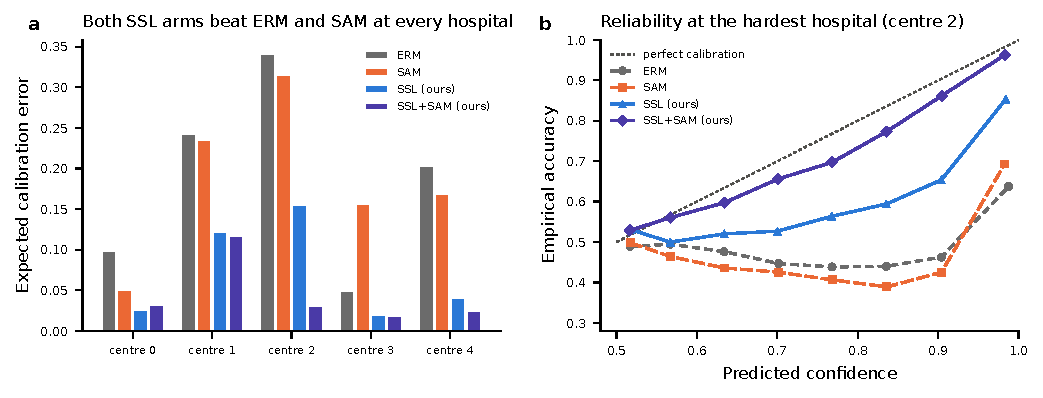
\includegraphics[width=\linewidth]{figs/fig4_calibration}
\caption{\textbf{(a)} Expected calibration error at each held-out hospital,
seed-averaged. \textbf{(b)} Reliability at the hardest hospital (centre 2),
three seeds pooled, 15 equal-width bins. ERM and SAM are anti-calibrated
over most of the range: higher confidence, lower accuracy.}
\label{fig:calib}
\end{figure}

%% ----------------------------------------------------------------
%% 5.4  OUT-OF-PARTITION
%% ----------------------------------------------------------------
\subsection{Out-of-partition validation on PatchCamelyon}
\label{sec:pcam}

A site-complete result inside Camelyon17-WILDS could still be a property of
that partition. We therefore evaluated all 60 checkpoints of the multi-seed
grid (5 folds $\times$ 4 arms $\times$ 3 seeds) on the $32{,}768$-patch
PatchCamelyon test split \citep{veeling2018pcam}, a different partition of the
Camelyon cohort, with no further training, model selection or tuning.
Table~\ref{tab:pcam} and Figure~\ref{fig:pcam} give the result.

\begin{table}[t]
\centering
\caption{Out-of-partition validation on PatchCamelyon. Statistics are computed
across the five WILDS folds after averaging the three seeds within each fold.
No PatchCamelyon example was seen in training, model selection or tuning.}
\label{tab:pcam}
\small
\begin{tabular}{lccccc}
\toprule
Arm & Mean AUROC & Across-fold SD & Worst fold & Best fold & ECE \\
\midrule
ERM     & $0.707$ & $0.095$ & $0.541$ & $0.768$ & $0.294$ \\
SAM     & $0.722$ & $0.092$ & $0.562$ & $0.798$ & $0.300$ \\
SSL     & $0.753$ & $0.046$ & $0.676$ & $0.786$ & $0.258$ \\
SSL+SAM & $\mathbf{0.779}$ & $\mathbf{0.014}$ & $\mathbf{0.762}$ & $0.797$ & $\mathbf{0.225}$ \\
\bottomrule
\end{tabular}
\end{table}

The absolute AUROC drops sharply, from $0.94$ in cohort to $0.78$. We take that
as a sobering measure of how little a $0.58$\,M-parameter model trained at
$64\times64$ transfers, and we return to it in \S\ref{sec:discussion}. The
structure of the result nonetheless reproduces. The across-fold standard
deviation falls from $0.095$ (ERM) to $0.014$ (SSL+SAM), a $6.8\times$
compression that is \emph{larger} than the $2.9\times$ seen within WILDS, and
the worst fold rises by $0.221$ AUROC, again larger than the in-cohort floor
lift of $0.169$. The calibration ordering is preserved too. Whatever
pre-training is doing, it is a property of the learned representation and not
of the WILDS partition.

\begin{figure}[t]
\centering
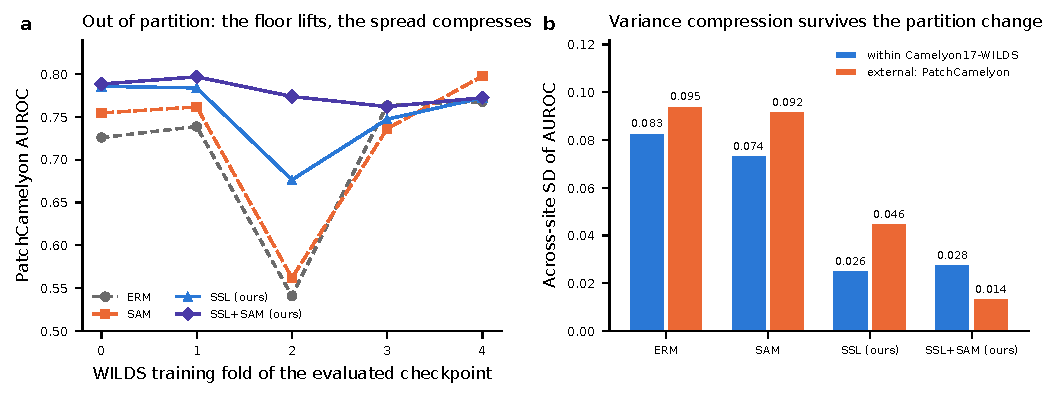
\includegraphics[width=\linewidth]{figs/fig3_external_pcam}
\caption{\textbf{(a)} PatchCamelyon AUROC of every checkpoint group, by the
WILDS fold it was trained on. \textbf{(b)} Across-site standard deviation
within WILDS and on PatchCamelyon. The compression relative to ERM survives the
partition change and strengthens for SSL+SAM.}
\label{fig:pcam}
\end{figure}

%% ----------------------------------------------------------------
%% 5.5  THE TWIST: ranking depends on shift type
%% ----------------------------------------------------------------
\subsection{The method ranking depends on the kind of shift}
\label{sec:cohorts}

Everything so far rests on one cohort, and Camelyon17's site variable bundles
three things together: the scanner, the staining and the patient population. A
natural question is which of the three the effect comes from, and whether any
of the conclusions above are properties of Camelyon17 rather than of
cross-domain evaluation. We therefore repeated the whole grid on two cohorts
where the scanner is the \emph{only} thing that varies.

\textbf{MIDOG 2021} \citep{aubreville2023midog} is 200 breast-cancer regions,
50 from each of four scanners, every one of them prepared in the same
laboratory. Three scanners carry annotations, which are binary: mitotic figure
versus a hard non-mitotic look-alike. Discriminating those two is the second
stage of the pipeline that won both MIDOG 2021 and 2022
\citep{jahanifar2024mitosis}, so the task sits inside the published problem.
Holding the lab constant removes the staining and preparation component of site
and leaves the acquisition device. $K=3$ labelled scanners is one short of
what the Camelyon17 protocol needs, so there is no spare domain to validate on
and epochs are selected on a held-out split of the two training scanners; and
because MIDOG carries about 2.8k training patches per fold rather than 30k, we
match total optimizer steps (50 epochs) instead of epochs. Everything else is
unchanged.

\textbf{Canine SCC} \citep{wilm2023canine} is 44 canine cutaneous squamous cell
carcinoma slides, each digitized on five scanners, with tumour and six tissue
classes annotated once and transferred to the other four scanners by
registration. We classify tumour against non-tumour tissue. This cohort is the
one place where the Camelyon17 protocol transfers with no adaptation at all:
$K=5$ domains, a genuine held-out validation scanner, and 24.5k--28.6k training
patches per fold, so the same five-epoch schedule applies. Two details matter.
The scanners differ in resolution, so a fixed pixel crop would make part of the
``domain effect'' a trivial zoom; because the annotations are registered, the
total annotated area per slide gives a precise scale ratio (coefficient of
variation $0.001$ across slides, matching the scanners' published
\textmu m/px), and we crop each scanner at its own pixel size and resize, so
patches cover a constant physical extent. And since the same 44 slides appear
under all five scanners, we also partition slides into five disjoint groups, so
a held-out fold withholds a scanner \emph{and} a set of slides, as a held-out
hospital in Camelyon17 withholds patients.

We also added the two published MIDOG top performers as arms, which brings the
grid to fifteen: \textbf{TIA-style}, the stain normalization plus heavy colour
and orientation augmentation of the challenge-winning classification stage
\citep{jahanifar2024mitosis}, and \textbf{RotInv}, the dihedral-invariance and
hard-negative strategy of \citet{lafarge2021rotation}.

\begin{table}[t]
\centering
\caption{The same grid on three cohorts, all through one pipeline and one
aggregator. $\sigma_{\mathrm{site}}$ and $\sigma_{\mathrm{run}}$ are the ERM
variance components; $K_{0.10}$ is the number of domains needed to detect a
$0.10$ AUROC mean effect at three seeds. Full per-arm tables are in
Appendix~\ref{app:cohorts}.}
\label{tab:cohorts}
\small
\begin{tabular}{llccccccc}
\toprule
Cohort & Domain is & $K$ & $\sigma_{\mathrm{site}}$ & $\sigma_{\mathrm{run}}$
& $\mathrm{ICC}$ & Best arm (worst-site) & SSL effect & $K_{0.10}$ \\
\midrule
Camelyon17 & hospital           & 5 & $0.074$ & $0.068$ & $0.55$ & Frozen probe $0.929$ & $+0.096^{*}$ & $8$ \\
MIDOG 2021 & scanner, one lab   & 3 & $\mathbf{0.025}$ & $0.039$ & $0.30$ & Macenko $0.865$      & $+0.028$ & $4$ \\
Canine SCC & scanner, 5 devices & 5 & $0.050$ & $0.040$ & $0.61$ & Frozen probe $0.792$ & $+0.012$ & $5$ \\
\bottomrule
\end{tabular}
\\[2pt]
{\footnotesize $^{*}$the only cohort where the SSL mean effect is significant
at $\alpha=0.05$ ($p=0.045$; MIDOG $p=0.17$, canine $p=0.43$).}
\end{table}

Table~\ref{tab:cohorts} and Figures~\ref{fig:cohortvar} and
\ref{fig:cohortrank} give the result, and it splits cleanly in two.

\paragraph{The design conclusions replicate; the method ranking does not.}
Both design claims hold on all three cohorts. Every cohort needs more
than one domain---$K_{0.10}$ is 8, 4 and 5 at three seeds, never 1---and on
every cohort a sizeable share of the variance is not site: the intraclass
correlation is $0.55$, $0.30$ and $0.61$, and on MIDOG the run-to-run term
$\sigma_{\mathrm{run}}=0.039$ actually \emph{exceeds} the between-scanner term
$\sigma_{\mathrm{site}}=0.025$. Fish and GroupDRO sit near the bottom of all
three tables. But the magnitude of the domain effect tracks what varies: ERM's
between-domain SD falls from $0.074$ when the domain is a hospital to $0.050$
and $0.025$ when it is only a scanner (Figure~\ref{fig:cohortvar}a). On this
evidence the scanner accounts for perhaps a third to two thirds of the
Camelyon17 hospital effect, and stain, preparation and case mix account for the
rest.

\paragraph{Stain normalization and the frozen probe swap places.}
Macenko stain normalization is eleventh of thirteen on Camelyon17 and
\emph{first of fifteen} on MIDOG, where it reaches worst-scanner AUROC $0.865$
against ERM's $0.754$. The frozen ImageNet probe is first on Camelyon17 and
first on canine but ninth on MIDOG. Figure~\ref{fig:cohortrank}a plots the
whole reordering. Both reversals make mechanistic sense once stated: MIDOG's
shift is purely one device's colour rendition of the same physical slide, which
is exactly what stain normalization is built to undo, whereas the frozen
ImageNet features that separate tumour from normal tissue so well carry little
about the fine nuclear morphology that distinguishes a mitotic figure from its
look-alike. The practical consequence is uncomfortable and worth stating
plainly: a method's robustness ranking cannot be read off one benchmark even
when that benchmark is evaluated domain-completely, because the \emph{kind} of
shift matters as much as which domain is held out.

\paragraph{Our own positive claim narrows.} The SSL mean effect is $+0.096$
AUROC on Camelyon17 ($p=0.045$), $+0.028$ on MIDOG ($p=0.17$) and $+0.012$ on
canine ($p=0.43$); SSL's rank by worst domain goes from second to fifth to
fourth (Figure~\ref{fig:cohortrank}b). Pre-training on in-domain unlabelled
tissue earns its cost when the shift includes a change of laboratory and
patient population, and not when the shift is only the acquisition device. That
is consistent with the NCT-CRC-HE result in Appendix~\ref{app:crc}, where a
same-institution stain perturbation also failed to reward pre-training, and it
replaces the broad claim we would have made from Camelyon17 alone with a
narrower one we can actually support. What does hold up across both scanner
cohorts is the published MIDOG-winning recipe: TIA-style is second by
worst-domain AUROC on MIDOG \emph{and} on canine, and the best-calibrated
trained-from-scratch arm on both.

\begin{figure}[t]
\centering
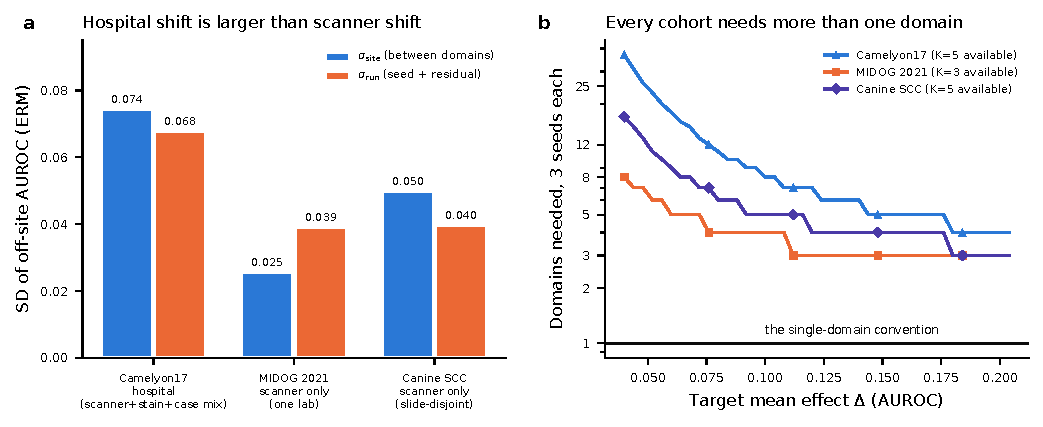
\includegraphics[width=\linewidth]{figs/fig6_cohort_variance}
\caption{\textbf{(a)} ERM variance components per cohort. The between-domain
term shrinks as the domain variable narrows from a hospital to a scanner, while
the run-to-run term stays put and on MIDOG overtakes it. \textbf{(b)} Domains
needed for $80\%$ power at three seeds. No cohort is served by one.}
\label{fig:cohortvar}
\end{figure}

\begin{figure}[t]
\centering
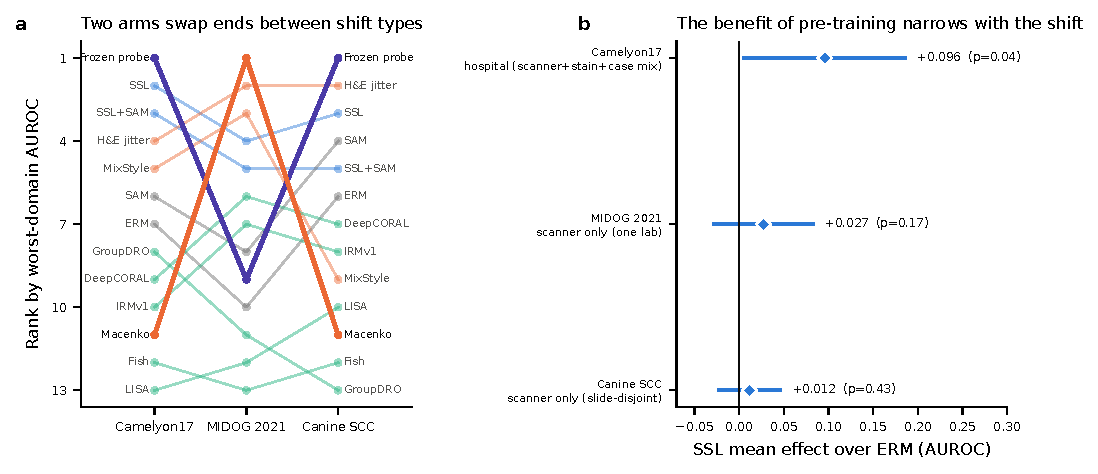
\includegraphics[width=\linewidth]{figs/fig7_cohort_ranking}
\caption{\textbf{(a)} Rank by worst-domain AUROC across the three cohorts, for
the thirteen arms common to all. Macenko (orange) and the frozen probe
(violet), highlighted, swap ends between hospital shift and scanner-only shift.
\textbf{(b)} SSL mean effect over ERM with a paired 95\% interval across
domains. The advantage is confined to the cohort whose domains differ by more
than the scanner.}
\label{fig:cohortrank}
\end{figure}

%% ----------------------------------------------------------------
%% 5.6  DESIGN RULES: variance decomposition
%% ----------------------------------------------------------------
\subsection{How many domains and seeds does an evaluation need?}
\label{sec:variance}

It would be tempting to read the results above as evidence that the test
hospital dominates everything. The seed-level detail in Table~\ref{tab:grid}
says otherwise. SAM's seed standard deviation at centre~3 is $0.278$
AUROC---reruns of one configuration at one hospital move the result further
than the entire across-hospital range of the baseline. Fitting the two-way
random-effects model $y_{ts} = \mu + b_t + e_{s(t)}$ to each arm
\citep{searle1992variance} separates the two sources (Table~\ref{tab:var},
Figure~\ref{fig:var}a).

\begin{table}[t]
\centering
\caption{Variance components of off-site AUROC, estimated per arm from the
$5\times3$ grid under $y_{ts}=\mu+b_t+e_{s(t)}$.
$\mathrm{ICC}_{\mathrm{site}}=\sigma^2_{\mathrm{site}}/(\sigma^2_{\mathrm{site}}+\sigma^2_{\mathrm{seed}}+\sigma^2_{\mathrm{resid}})$
is the share of variance attributable to hospital identity.}
\label{tab:var}
\small
\begin{tabular}{lcccc}
\toprule
Arm & $\sigma_{\mathrm{site}}$ & $\sigma_{\mathrm{seed}}$ & $\sigma_{\mathrm{resid}}$ & $\mathrm{ICC}_{\mathrm{site}}$ \\
\midrule
ERM     & $0.074$ & $0.019$ & $0.065$ & $0.55$ \\
SAM     & $0.028$ & $0.056$ & $0.119$ & $\mathbf{0.04}$ \\
SSL     & $0.020$ & $0.000$ & $0.027$ & $0.36$ \\
SSL+SAM & $0.028$ & $0.000$ & $0.012$ & $0.84$ \\
\bottomrule
\end{tabular}
\end{table}

Hospital identity accounts for $55\%$ of the baseline's variance and only $4\%$
of SAM's (Table~\ref{tab:var}). So single-hospital, single-seed evaluation is
under-powered in two directions at once, and averaging more seeds does not
substitute for adding hospitals any more than the reverse does. The
decomposition is also useful diagnostically. SAM's across-site standard
deviation of $0.074$ looks comparable to the baseline's, but almost none of it
is systematic site structure: the spread is instability, not site sensitivity.

\begin{figure}[t]
\centering
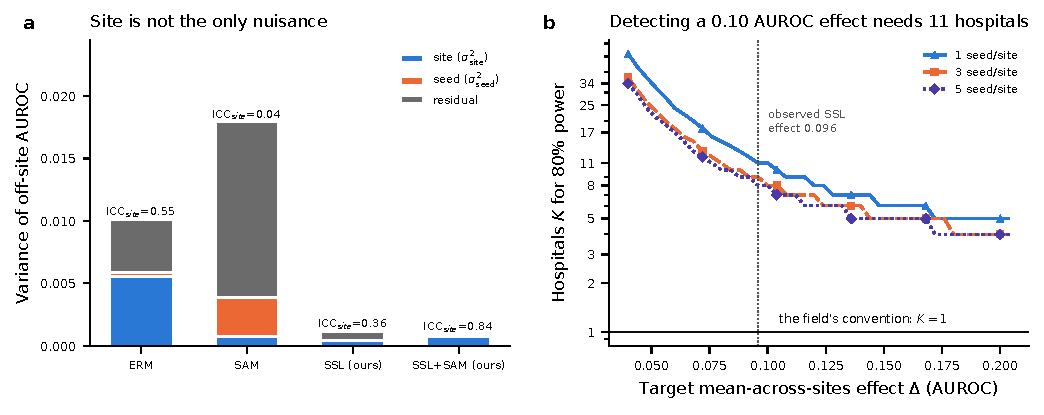
\includegraphics[width=\linewidth]{figs/fig2_variance_power}
\caption{\textbf{(a)} Variance of off-site AUROC decomposed into site, seed and
residual components. SAM's variance is almost entirely non-site;
SSL+SAM's is almost entirely site, at one eighth the magnitude.
\textbf{(b)} Hospitals required for $80\%$ power at $\alpha=0.05$ as a
function of the target mean effect, under the baseline's variance components.}
\label{fig:var}
\end{figure}

\paragraph{How many hospitals is enough.} Under the same model, the standard
error of a mean-across-sites contrast from a $K$-hospital, $s$-seed design is
$\sqrt{\sigma^2_{\mathrm{site}}/K + \sigma^2_{\mathrm{run}}/(Ks)}$, where
$\sigma_{\mathrm{run}}$ collects the seed and residual terms. Solving for the
smallest $K$ at which a paired $t$-test reaches $80\%$ power gives
Table~\ref{tab:power} and Figure~\ref{fig:var}b. Detecting a $0.10$ AUROC mean
effect needs eleven hospitals at one seed each, or eight at three seeds.
Camelyon17 provides five. A single-hospital ablation reporting a mean effect
below roughly $0.20$ AUROC is therefore under-powered by an order of magnitude.
This is also why we prefer the worst-site and across-site-spread summaries:
they say something at $K=5$, whereas the mean does not.

\begin{table}[t]
\centering
\caption{Hospitals $K$ needed to detect a mean-across-sites effect $\Delta$
with $80\%$ power at $\alpha=0.05$ (two-sided), under
$\sigma_{\mathrm{site}}=0.074$ and $\sigma_{\mathrm{run}}=0.068$ estimated
from the baseline arm of this grid.}
\label{tab:power}
\small
\begin{tabular}{lccccc}
\toprule
$\Delta$ (AUROC) & $0.05$ & $0.075$ & $0.10$ & $0.15$ & $0.20$ \\
\midrule
$K$, 1 seed/site  & $34$ & $17$ & $11$ & $6$ & $5$ \\
$K$, 3 seeds/site & $25$ & $12$ & $8$  & $5$ & $4$ \\
$K$, 5 seeds/site & $23$ & $12$ & $8$  & $5$ & $4$ \\
\bottomrule
\end{tabular}
\end{table}

%% ================================================================
%%  DISCUSSION
%% ================================================================
\section{Discussion}
\label{sec:discussion}

\paragraph{Why domain shift type matters more than domain shift magnitude.}
The most important finding in this paper is not that single-hospital evaluation
is unreliable---that is the premise---but that the \emph{kind} of shift
between domains governs which method works. Hospital shift bundles three
distinct sources: scanner hardware, staining chemistry, and patient/case-mix
variation. When all three change together (Camelyon17), the effective
intervention is one that builds a more general representation---self-supervised
pre-training or aggressive augmentation---because no single normalization step
can undo a compound shift. When only the scanner changes (MIDOG, canine
cohort), stain normalization removes the dominant signal directly and nothing
else is needed. The frozen-probe result sharpens this further: a
general-purpose ImageNet representation already encodes enough about tissue
structure that it is largely invariant to hospital-level confounds, which
explains why it ranks first under hospital shift but drops under scanner-only
shift, where the task (mitosis classification) demands fine morphological
features that ImageNet representations do not capture. For developers building
clinical AI, the implication is that robustness is not a single axis with a
single solution. The first step is to characterize the deployment shift---is it
a scanner change, a protocol change, or a full institutional change?---and
then select the intervention that addresses that specific source.

\paragraph{The ICC as a design tool for robustness evaluation.}
Current evaluation practice treats site as the only nuisance variable. Our
variance decomposition shows this is incomplete: on the supervised baseline,
hospital identity accounts for $55\%$ of the variance
($\mathrm{ICC}_{\mathrm{site}}=0.55$), but on SAM it accounts for only $4\%$;
the rest is seed and residual noise. Without the decomposition, SAM's
across-site SD of $0.074$ looks comparable to the baseline's $0.083$, but the
ICC reveals that SAM's spread is instability rather than site sensitivity---a
distinction invisible to any summary that does not separate the two sources.
The ICC also provides a direct path to statistical power. Our closed-form
expression for the standard error of a mean-across-sites contrast yields a
concrete design rule: detecting a $0.10$ AUROC effect at $80\%$ power requires
eight hospitals at three seeds. Camelyon17's five hospitals fall short, which is
why we recommend worst-site and across-site spread as primary summaries: they
remain informative at $K=5$ where the mean does not. We propose that future
robustness papers report the ICC alongside their accuracy numbers, so that
readers can judge whether the evaluation grid is powered to support the claimed
effect.

\paragraph{Implications for clinical AI deployment.}
For companies and hospitals developing pathology AI for multi-site deployment,
our results suggest a three-step workflow. First, \emph{characterize the
shift}: determine whether the target sites differ from the training sites in
scanner, staining protocol, patient population, or all three. Second,
\emph{select the intervention accordingly}: use stain normalization for
scanner-only shifts; use self-supervised pre-training or strong
colour/stain augmentation for full institutional shifts; invest in stronger
backbone representations when possible, since the frozen-probe result shows
this is the most effective single lever. Third, \emph{validate
domain-completely}: run the model at every available site rather than one,
report worst-site performance as the deployment-relevant metric, replicate
seeds, and compute the ICC to verify that the evaluation has sufficient power.
The protocol costs under one hour of GPU time at compact-model scale---less
than a single conventional ablation.

\paragraph{What the grid corrected in our own work.}
Three findings contradicted what we expected. The hospital effect is not the
dominant nuisance: once seeds are replicated, random variation accounts for
roughly half the total variance, and on MIDOG it exceeds the hospital effect.
A gain-versus-baseline diagnostic we had used to argue that our method targets
the hard hospitals is negative by construction (Appendix~\ref{app:shape}): any
uniformly better method produces the same pattern with no actual targeting.
And the cross-cohort comparison undercut the method ranking we would have
published from Camelyon17 alone. All three corrections fell out of running the
evaluation completely and repeating it on data with a different shift structure.

\paragraph{Caveats.}
The most important caveat is model scale. Every trained arm uses a $0.58$\,M-parameter
CNN at $64\times64$ resolution, which makes the protocol affordable but limits
how far the conclusions generalize. The frozen-probe result suggests that
larger representations may dissolve the hospital-to-hospital gap entirely;
whether the patterns we report survive fine-tuning of a pathology foundation
model \citep{chen2024uni} is the most important open question. PatchCamelyon,
our out-of-partition test, shares the consortium and scanners with our training
data and is therefore not truly independent external validation; the absolute
AUROC values ($0.71$--$0.78$) confirm that these are comparative instruments,
not deployment-ready models. Pre-training only helps under institutional shift:
on NCT-CRC-HE (Appendix~\ref{app:crc}), where the shift is a
same-institution stain perturbation, every intervened arm underperforms the
baseline. Appendix~\ref{app:caveats} collects further caveats including
re-implementation fidelity, non-independent folds, and unmatched compute
budgets.

%% ================================================================
%%  CONCLUSION
%% ================================================================
\section{Conclusion}

Cross-domain generalization in histopathology is not a single problem with a
single solution. By running eleven methods across three cohorts that isolate
different sources of shift, we show that the type of domain
difference---scanner, staining protocol, or full institutional change---determines
which robustness strategy succeeds and which fails. Under hospital shift,
self-supervised pre-training compresses the across-site spread threefold and
raises the worst hospital by $0.175$ AUROC; under scanner-only shift, stain
normalization dominates and pre-training adds nothing. Most
domain-generalization objectives hurt the worst domain across all three
cohorts. A frozen ImageNet probe outperforms every trained-from-scratch arm
under hospital shift, establishing representation quality as a stronger lever
than any robustness objective at this scale.

We propose using the intraclass correlation coefficient from a variance
decomposition of off-site performance as the field's standard measure for
evaluating robustness claims. This single statistic separates true site
sensitivity from seed noise, yields a closed-form power calculation for
experimental design, and exposes under-powered evaluations before they produce
misleading conclusions.

For the development of clinical pathology AI with practical cross-domain
generalization: characterize the deployment shift before choosing an
intervention, validate domain-completely at every available site, report
worst-site performance as the deployment-relevant metric, replicate seeds, and
use the ICC to verify that the evaluation grid supports the claimed effect. The
complete protocol costs under one hour of GPU time---there is no computational
barrier to doing this correctly.

\subsubsection*{Broader impact statement}

This work uses only de-identified public data releases; no new patient data
were collected and no ethics approval was required. Its direct intent is to
make cross-hospital robustness claims in medical imaging harder to overstate,
which we view as a safety contribution. The models reported here are research
instruments trained at reduced resolution with low absolute accuracy and are
explicitly not suitable for clinical use; we flag this because released
checkpoints in this area are sometimes reused out of context.

\subsubsection*{Reproducibility statement}

Camelyon17-WILDS \citep{koh2021wilds} and PatchCamelyon \citep{veeling2018pcam}
are public under CC0; NCT-CRC-HE and CRC-VAL-HE-7K
\citep{kather2018nct,kather2019predicting} are public under CC-BY; MIDOG 2021
\citep{aubreville2023midog} and the multi-scanner canine cohort
\citep{wilm2023canine} are public on Zenodo under CC-BY. Code, the
fold-materialization scripts for all four cohorts, the per-run JSON records for
all 388 GPU jobs, the variance-decomposition and power code, and the single
script that regenerates every table and figure in this paper from those records
are available at
\url{https://github.com/InvenTide-AI/histopath-shift}.

\bibliography{main}
\bibliographystyle{tmlr}

\appendix
\section{Further caveats}
\label{app:caveats}

\paragraph{Re-implementation fidelity.} Our Fish and LISA arms are not the code
the original authors ran. They were given no per-arm tuning, they sit inside a
$0.58$\,M-parameter five-epoch pipeline rather than the DenseNet-scale setups
of the original papers, and in Fish's case the out-of-distribution validation
curve selects epoch 1 in four of five folds
(Figure~\ref{fig:supp_epoch}). Table~\ref{tab:eleven} is thirteen arms under
one fixed protocol, not a ranking of these methods at their best. Our claim
about them concerns how much their off-site accuracy moves when the held-out
hospital changes, which is a property of the protocol and not of the
implementation.

\paragraph{The folds are not independent draws.} Each of the five centres
appears in three of the five training sets, so the folds share training data
and the fold-level intervals we report are approximate and mildly optimistic.
The power calculation in \S\ref{sec:variance} inherits the same approximation.
A cohort with more centres would let the grid be built from disjoint training
sets; Camelyon17 does not.

\paragraph{Compute is not matched.} The pre-trained arms consume additional
unlabelled data and additional optimization steps that the supervised arms do
not, and the frozen-probe arm rests on an ImageNet-1K pre-training budget that
is not counted anywhere in our totals. A compute-matched control, and an
augmentation-only control using the same colour and stain jitter without the
contrastive objective, would separate the representation learning from the
extra budget. We ship both as scripts but have not run them at the full grid.

\section{Per-arm, per-hospital results}
\label{app:full}

Figure~\ref{fig:supp_heat} gives every arm at every hospital. The ordering of
arms changes substantially from hospital to hospital, which is the paper's
central practical point in one picture: at centre 0 all thirteen arms fall
within $0.106$ AUROC of one another, while at centre 2 the same thirteen arms
span $0.420$.

\begin{figure}[h]
\centering
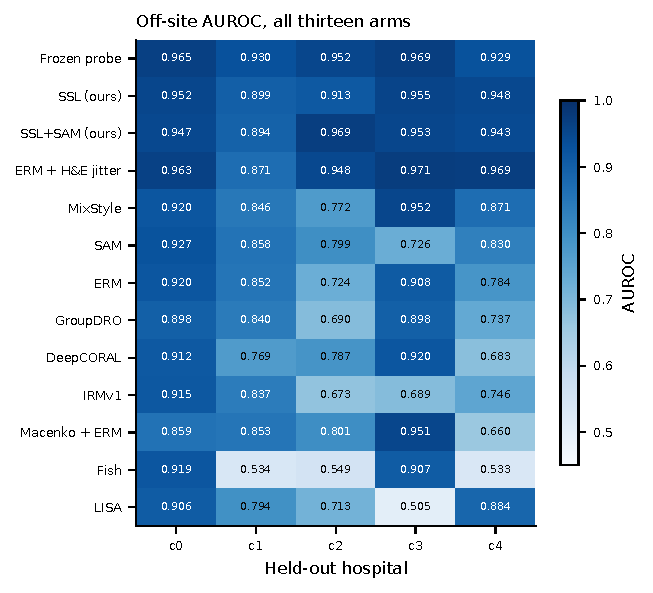
\includegraphics[width=0.72\linewidth]{figs/figS1_heatmap}
\caption{Off-site test AUROC for all thirteen arms at all five held-out
hospitals, seed-averaged where multiple seeds were run.}
\label{fig:supp_heat}
\end{figure}

Figure~\ref{fig:supp_seed} shows every individual run of the four core arms,
making the seed spread visible without summary statistics.

\begin{figure}[h]
\centering
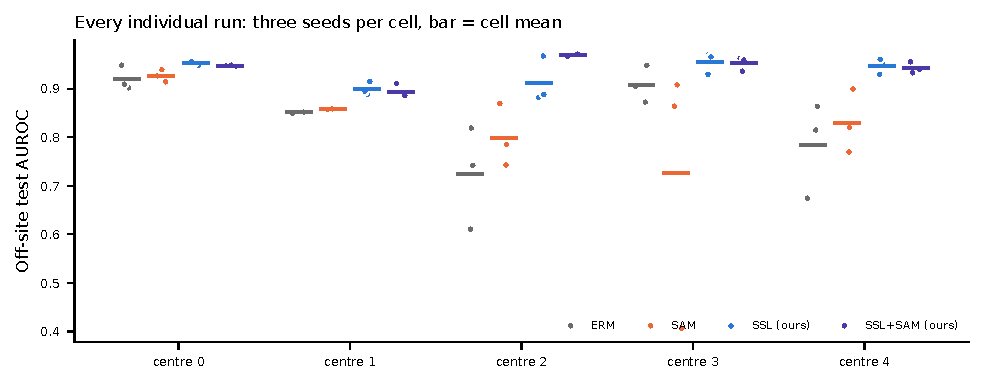
\includegraphics[width=\linewidth]{figs/figS2_seedspread}
\caption{All 60 individual runs of the four core arms. Horizontal bars are cell
means. The baseline's spread at centres 2 and 4, and SAM's at centre 3, are
seed effects rather than site effects.}
\label{fig:supp_seed}
\end{figure}

\begin{figure}[h]
\centering
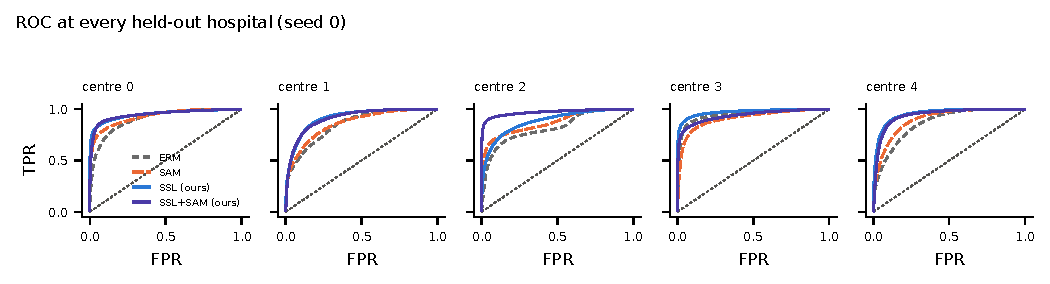
\includegraphics[width=\linewidth]{figs/figS3_roc}
\caption{ROC curves at every held-out hospital, seed 0.}
\label{fig:supp_roc}
\end{figure}

\begin{figure}[h]
\centering
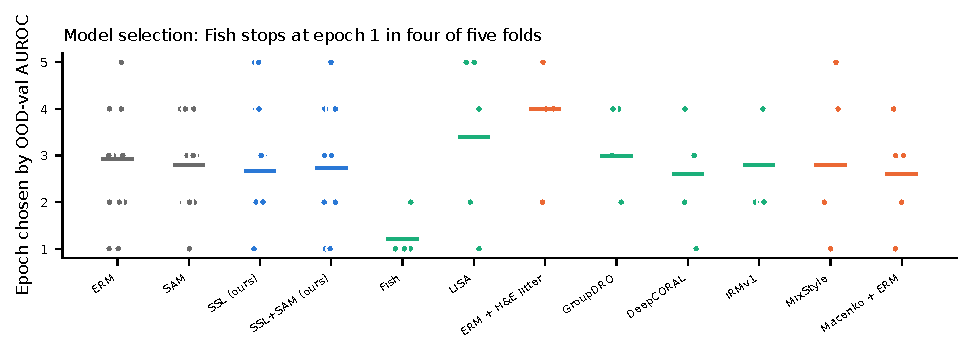
\includegraphics[width=\linewidth]{figs/figS4_selected_epoch}
\caption{Epoch selected by out-of-distribution validation AUROC, every run.
Fish selects epoch 1 in four of five folds, which contributes to its low
worst-site score in Table~\ref{tab:eleven} and should be read as a
model-selection pathology under our protocol rather than as a property of the
method.}
\label{fig:supp_epoch}
\end{figure}

\section{Full per-arm tables for the two scanner cohorts}
\label{app:cohorts}

Columns match Table~\ref{tab:eleven}. Both cohorts were run through the same
pipeline, the same arm code and the same aggregator as Camelyon17; the
aggregator reproduces the Camelyon17 numbers in Table~\ref{tab:eleven} exactly
when pointed at that cohort's records.

\begin{table}[h]
\centering
\caption{MIDOG 2021, scanner-complete, $K=3$. Mitotic figure versus annotated
non-mitotic look-alike, all 150 annotated regions. Ordered by worst-scanner
AUROC. Note Macenko at the top and the frozen probe in tenth: both are the
reverse of their Camelyon17 positions.}
\label{tab:midog_full}
\small
\setlength{\tabcolsep}{4pt}
\begin{tabular}{lcccccccc}
\toprule
Arm & Worst & SD & Mean & Seed SD & ECE & $r$ & $r_0$ & $r-r_0$ \\
\midrule
Macenko + ERM       & $\mathbf{0.865}$ & $\mathbf{0.013}$ & $0.880$ & --- & $0.078$ & $-0.93$ & $-0.93$ & $+0.00$ \\
TIA-style           & $0.860$ & $0.022$ & $\mathbf{0.885}$ & --- & $\mathbf{0.053}$ & $-0.75$ & $-0.83$ & $+0.08$ \\
ERM + H\&E jitter   & $0.834$ & $0.026$ & $0.863$ & --- & $0.058$ & $-0.60$ & $-0.78$ & $+0.18$ \\
MixStyle            & $0.790$ & $0.010$ & $0.799$ & --- & $0.265$ & $-1.00$ & $-0.95$ & $-0.04$ \\
SSL (ours)          & $0.789$ & $0.018$ & $0.807$ & $0.022$ & $0.226$ & $-0.85$ & $-0.88$ & $+0.03$ \\
SSL+SAM (ours)      & $0.783$ & $0.016$ & $0.798$ & $0.015$ & $0.277$ & $-0.98$ & $-0.89$ & $-0.08$ \\
DeepCORAL           & $0.776$ & $0.033$ & $0.813$ & --- & $0.227$ & $-0.45$ & $-0.71$ & $+0.25$ \\
IRMv1               & $0.775$ & $0.033$ & $0.800$ & --- & $0.244$ & $+0.58$ & $-0.70$ & $+1.28$ \\
SAM                 & $0.765$ & $0.029$ & $0.784$ & $0.018$ & $0.268$ & $-0.51$ & $-0.75$ & $+0.24$ \\
Frozen probe        & $0.756$ & $0.012$ & $0.768$ & --- & $0.075$ & $-0.93$ & $-0.94$ & $+0.00$ \\
ERM baseline        & $0.754$ & $0.033$ & $0.779$ & $0.034$ & $0.240$ & --- & --- & --- \\
GroupDRO            & $0.750$ & $0.034$ & $0.783$ & --- & $0.293$ & $-0.06$ & $-0.70$ & $+0.63$ \\
RotInv              & $0.732$ & $0.059$ & $0.788$ & --- & $0.275$ & $+0.88$ & $-0.49$ & $+1.36$ \\
LISA                & $0.680$ & $0.061$ & $0.750$ & --- & $0.309$ & $+0.26$ & $-0.48$ & $+0.73$ \\
Fish                & $0.578$ & $0.054$ & $0.637$ & --- & $0.173$ & $-0.52$ & $-0.52$ & $+0.01$ \\
\bottomrule
\end{tabular}
\end{table}

\begin{table}[h]
\centering
\caption{Canine multi-scanner SCC, scanner-complete, $K=5$, scale-normalized
and slide-disjoint. Tumour versus non-tumour tissue. This is the one cohort
where the Camelyon17 protocol applies without adaptation.}
\label{tab:canine_full}
\small
\setlength{\tabcolsep}{4pt}
\begin{tabular}{lcccccccc}
\toprule
Arm & Worst & SD & Mean & Seed SD & ECE & $r$ & $r_0$ & $r-r_0$ \\
\midrule
Frozen probe        & $\mathbf{0.792}$ & $0.038$ & $\mathbf{0.845}$ & --- & $0.094$ & $-0.70$ & $-0.81$ & $+0.11$ \\
TIA-style           & $0.773$ & $0.034$ & $0.821$ & --- & $0.055$ & $-0.80$ & $-0.84$ & $+0.04$ \\
ERM + H\&E jitter   & $0.756$ & $\mathbf{0.029}$ & $0.777$ & --- & $\mathbf{0.043}$ & $-0.86$ & $-0.88$ & $+0.02$ \\
SSL (ours)          & $0.703$ & $0.038$ & $0.744$ & $0.037$ & $0.143$ & $-0.72$ & $-0.81$ & $+0.09$ \\
SAM                 & $0.702$ & $0.060$ & $0.744$ & $\mathbf{0.015}$ & $0.143$ & $-0.06$ & $-0.66$ & $+0.61$ \\
SSL+SAM (ours)      & $0.697$ & $0.047$ & $0.752$ & $0.032$ & $0.114$ & $-0.53$ & $-0.76$ & $+0.22$ \\
ERM baseline        & $0.694$ & $0.054$ & $0.733$ & $0.034$ & $0.198$ & --- & --- & --- \\
DeepCORAL           & $0.678$ & $0.054$ & $0.734$ & --- & $0.146$ & $-0.24$ & $-0.70$ & $+0.46$ \\
IRMv1               & $0.673$ & $0.061$ & $0.755$ & --- & $0.141$ & $-0.39$ & $-0.66$ & $+0.27$ \\
MixStyle            & $0.669$ & $0.082$ & $0.742$ & --- & $0.162$ & $+0.67$ & $-0.55$ & $+1.22$ \\
LISA                & $0.635$ & $0.071$ & $0.740$ & --- & $0.251$ & $-0.36$ & $-0.60$ & $+0.25$ \\
Macenko + ERM       & $0.615$ & $0.098$ & $0.733$ & --- & $0.139$ & $+0.33$ & $-0.48$ & $+0.81$ \\
Fish                & $0.603$ & $0.089$ & $0.715$ & --- & $0.156$ & $-0.23$ & $-0.51$ & $+0.28$ \\
RotInv              & $0.597$ & $0.081$ & $0.701$ & --- & $0.188$ & $+0.02$ & $-0.55$ & $+0.57$ \\
GroupDRO            & $0.518$ & $0.119$ & $0.697$ & --- & $0.155$ & $+0.36$ & $-0.41$ & $+0.77$ \\
\bottomrule
\end{tabular}
\end{table}

The excess response-shape statistic behaves the same way here as on
Camelyon17 and reinforces Appendix~\ref{app:shape}: the arms at the top of each table
sit at or near zero excess, meaning they are uniformly better rather than
selectively repairing weak domains, while GroupDRO, MixStyle, IRMv1 and RotInv
carry large positive excess on one cohort or the other, sending what gain they
have to the domains that were already handled.

\section{Second task: NCT-CRC-HE}
\label{app:crc}

To test whether the benefit of pre-training is specific to institutional shift
we repeated the four core arms on NCT-CRC-HE \citep{kather2018nct}, a
colorectal H\&E task (tumour epithelium versus all other tissue, tiles resized
to $64\times64$), with $20{,}000$ training and $4{,}000$ in-distribution
validation tiles from the colour-normalized release and $10{,}226$ further
tiles held unlabelled for pre-training (drawn from the colour-normalized
cohort only, so the encoder never sees the perturbed appearance that forms the
test condition). Two shift axes are available, neither of which is a change of
institution: a stain-appearance perturbation of the training tissue, and the
patient-disjoint CRC-VAL-HE-7K release from the same tissue bank
\citep{kather2019predicting}. Two seeds per arm. One protocol difference from
\S\ref{sec:protocol} is forced by the data: NCT-CRC-HE has no second site, so
epochs are selected on in-distribution validation rather than on a held-out
validation hospital.

\begin{table}[h]
\centering
\caption{NCT-CRC-HE, mean over two seeds. Neither shift axis is an institution
change, and on both the intervened arms fail to beat the baseline.}
\label{tab:crc}
\small
\begin{tabular}{lcccccc}
\toprule
& \multicolumn{2}{c}{In-distribution val} & \multicolumn{2}{c}{Stain perturbation} & \multicolumn{2}{c}{CRC-VAL-HE-7K} \\
\cmidrule(lr){2-3}\cmidrule(lr){4-5}\cmidrule(lr){6-7}
Arm & AUROC & ECE & AUROC & ECE & AUROC & ECE \\
\midrule
ERM     & $0.972$ & $0.010$ & $\mathbf{0.791}$ & $\mathbf{0.156}$ & $0.940$ & $\mathbf{0.027}$ \\
SAM     & $0.966$ & $0.017$ & $0.726$ & $0.206$ & $\mathbf{0.944}$ & $0.037$ \\
SSL     & $0.969$ & $0.011$ & $0.702$ & $0.235$ & $0.927$ & $0.032$ \\
SSL+SAM & $0.963$ & $0.017$ & $0.724$ & $0.232$ & $0.936$ & $0.036$ \\
\bottomrule
\end{tabular}
\end{table}

Table~\ref{tab:crc} is a clean negative result. On the stain-perturbation axis
SSL costs $0.089$ AUROC relative to the baseline; on the patient-disjoint
external cohort all four arms are within $0.017$ AUROC of one another, and the
baseline is better calibrated than any intervened arm on both axes. We read
this as a scope statement on \S\ref{sec:ssl}: pre-training on in-domain
unlabelled tissue earns its cost where the shift is a genuine change of
institution, and not where it is a same-institution appearance perturbation.
Because NCT-CRC-HE is single-institution, it also offers no site structure to
replicate over. It is a $K=1$ design by construction, and
Table~\ref{tab:power} applies to it.

\section{A finding of our own that the site-complete grid overturned}
\label{app:correction}

We record this because it motivated the study and because it illustrates the
protocol's value on our own work. An earlier single-hospital experiment of ours
at Camelyon17 centre 2 reported a synergy of $+0.161$ AUROC between
pre-training and sharpness-aware minimization, decomposed as
$\delta_{\mathrm{SSL}}=-0.037$, $\delta_{\mathrm{SAM}}=-0.105$ and
$I=+0.161$, and interpreted the interaction as a property of the method pair.

Under the site-complete grid that interpretation does not survive. The
interaction term has a five-hospital mean of $+0.017$ AUROC (95\% CI
$[-0.097,+0.132]$, $p=0.70$) and changes sign across hospitals
(Table~\ref{tab:grid}); at centre 2 itself, with three seeds instead of one, it
is $-0.019$. The original estimate was driven by a single anomalous SAM run:
because $I$ is a difference of four arm-level estimates, one bad cell
propagates into it undiminished, and SAM is the least stable arm in the study
(seed SD $0.084$, and $0.278$ at centre 3). The reading we now think correct is
that $+0.161$ described one hospital and one unlucky run, and the synergy claim
is withdrawn. What does survive is this paper's positive result: the worst-site
lift and the variance compression of pre-training itself, both of which are
larger and better supported under $K=5$ with three seeds than anything the
$K=1$ experiment could have established.

\section{The response-shape diagnostic}
\label{app:shape}

An intervention for site robustness ought to help most where the baseline fails
and little where it already succeeds. The natural way to check is the
correlation $r$ between an arm's per-hospital gain and the baseline's
per-hospital AUROC, and a large negative $r$ looks like evidence of exactly
that targeting. We used this statistic, and it is misleading.

Because the gain is $M - E$ and is correlated against $E$ itself, the statistic
is non-zero even when an arm's per-hospital performance is statistically
independent of the baseline's. For independent $M$ and $E$ with across-site
standard deviations $\sigma_M, \sigma_E$,
\[
\mathrm{Cov}(M-E,\,E) = -\sigma_E^2,
\qquad
r_0 \;=\; \frac{-\sigma_E^2}{\sigma_E\sqrt{\sigma_M^2+\sigma_E^2}}
\;=\; \frac{-\sigma_E}{\sqrt{\sigma_M^2+\sigma_E^2}} .
\]
An arm that is merely \emph{flat} across hospitals ($\sigma_M \to 0$) therefore
has $r_0 \to -1$ with no targeting whatever. Our own arms are exactly in that
regime: SSL has $r=-0.95$ against $r_0=-0.96$, and SSL+SAM $r=-0.96$ against
$r_0=-0.95$ (Table~\ref{tab:eleven}, Figure~\ref{fig:shape}). The excess is
zero to two decimal places. Our pre-trained arms do not preferentially repair
the hard hospitals; they are uniformly better, and the apparent targeting was
an artifact of the statistic.

Removing the null makes the statistic informative again, and what it finds is
the reverse of the naive reading. GroupDRO sits $+1.37$ above its null and Fish
$+0.97$: these arms concentrate what gain they have at the hospitals where the
baseline is \emph{already} strong, widening the cross-hospital gap they are
meant to close. DeepCORAL ($+0.51$), Macenko ($+0.46$), IRMv1 ($+0.35$) and
MixStyle ($+0.21$) show the same misallocation more mildly. We recommend
reporting $r - r_0$ with $r_0$ from Equation~\ref{eq:null}, and reporting it
alongside rather than instead of the worst-site value.

\begin{figure}[h]
\centering
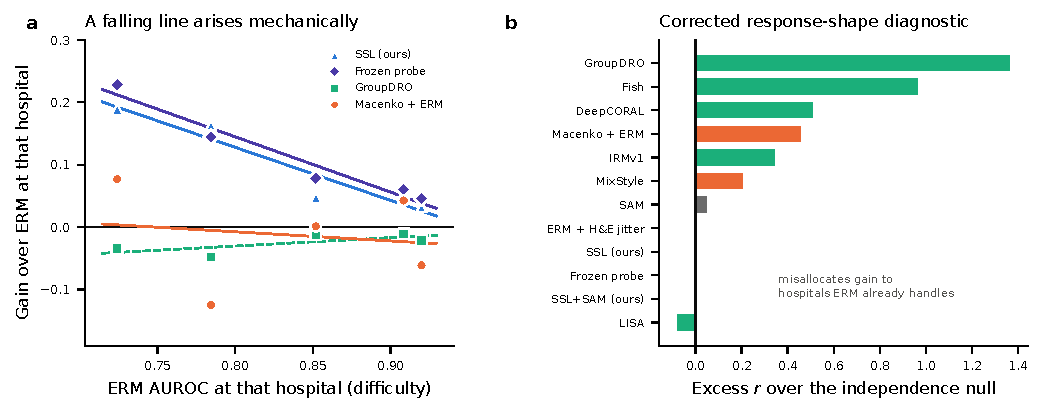
\includegraphics[width=\linewidth]{figs/fig5_response_shape}
\caption{\textbf{(a)} Per-hospital gain against per-hospital baseline
difficulty for one arm from each family. The pre-trained and frozen arms show
steep negative slopes; so would any arm with low across-site variance, by
Equation~\ref{eq:null}. \textbf{(b)} Excess correlation over the independence
null. Positive excess means the arm sends its gain to hospitals the baseline
already handles.}
\label{fig:shape}
\end{figure}

\end{document}
